Aufgrund einer Kopplung der beiden Gleichungen \ref{enq:Bewgltrans} und \ref{enq:Bewglrot} entsteht eine sogenannte algebraische Schleife, welche besagt:

\begin{center}
	Ursache gleich Wirkung gleich Ursache. \cite[S. 64]{HelmutBode.}
\end{center}

Durch eine Vereinfachung des Systems soll die algebraische Schleife verhindert werden. Dies wird mithilfe von Matlab SIMULINK durchgeführt. \\
Die Parameter werden mit den Funktionen \ref{enq:Spannungen}, \ref{enq:Bewgltrans}, \ref{enq:Bewglrot} und \ref{enq:Unwuchtkraft} in einem Blockdiagramm verknüpft. So vereinfacht sich zum einen das System, zum anderen kann man leichter eine Aussage über das Verhalten des Systems treffen.

\begin{figure}[hbt]
	\centering
	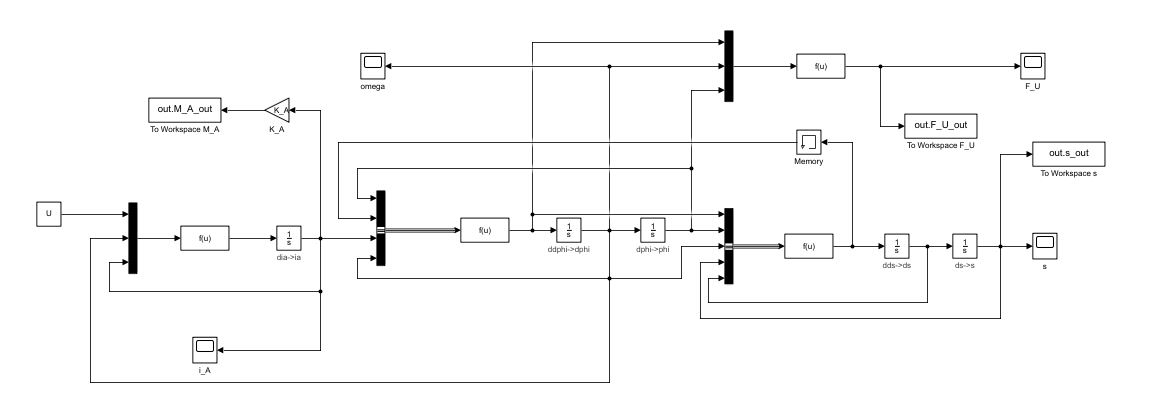
\includegraphics[width=1\linewidth]{Images/ProjektB_Elektrik_Blockdiagramm}
	\caption{Matlab SIMULINK Blockdiagramm zur Simulation des Systemverhaltens mit Memory-Block zur Umgehung der algebraischen Schleife}
	\label{fig:Blockdiagramm}
\end{figure}

\newpage

Als nächstes müssen die Variablen im Workspace angelegt werden. Diese sind wie folgt zu deklarieren: \\

\begin{figure}[hbt]
	\centering
	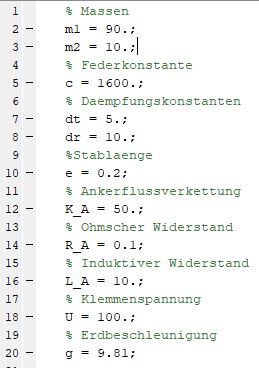
\includegraphics[width=0.3\linewidth]{Images/Variablen}
	\caption{Angelegte Variablen in Matlab im Workspace}
	\label{fig:Variablen}
\end{figure}

Damit Matlab SIMULINK die Variablen nicht selbst anlegt und mit Werten überschreibt, muss eine Referenz auf die Eingangsvariable $U$ des Workspaces im Model Explorer gesetzt werden. Falls die benötigten Variablen von SIMULINK schon angelegt wurden, muss diese über den Model Explorer gelöscht werden. Nun kann die Schaltung mit den richtigen Parametern simuliert werden.